\documentclass[tikz]{standalone}

\usepackage[T1]{fontenc}
\usepackage[english]{babel}

\usepackage{tikz}

\begin{document}
	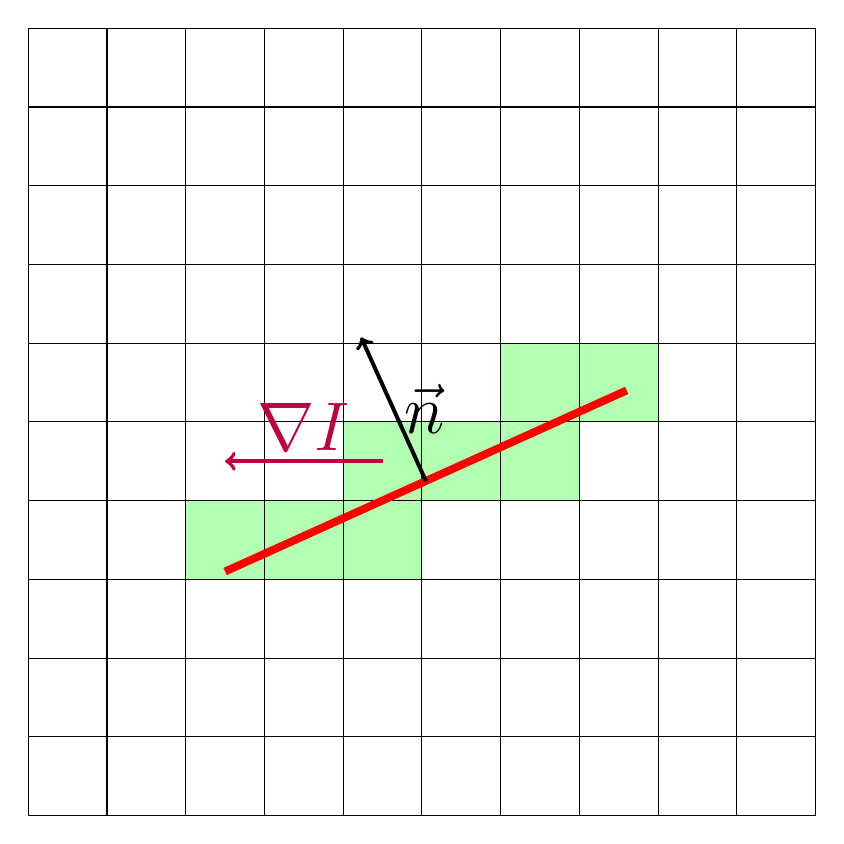
\begin{tikzpicture}
		\draw (0, 0) grid (10, 10);
		\draw[fill=green!30] (2, 3) rectangle (3, 4);
		\draw[fill=green!30] (3, 3) rectangle (4, 4);
		\draw[fill=green!30] (4, 3) rectangle (5, 4);
		\draw[fill=green!30] (4, 4) rectangle (5, 5);
		\draw[fill=green!30] (5, 4) rectangle (6, 5);
		\draw[fill=green!30] (6, 4) rectangle (7, 5);
		\draw[fill=green!30] (6, 5) rectangle (7, 6);
		\draw[fill=green!30] (7, 5) rectangle (8, 6);
		\draw[red, line width=1mm] (2.5, 3.1) -- (7.6, 5.4);
		\draw[black, line width=.5mm, ->] (5.05, 4.25) -- (4.227784494, 6.073173514) node[midway, right] {\Huge $\vec{n}$};
		\draw[purple, line width=.5mm, ->] (4.5, 4.5) -- (2.5, 4.5) node[midway, above] {\Huge \bf $\nabla I$};
	\end{tikzpicture}
\end{document}
